\documentclass[tikz,border=8pt]{standalone}
\usepackage{amsmath}
\usepackage{amssymb}
\usetikzlibrary{
    arrows.meta,
    backgrounds,
    calc,
    decorations.pathmorphing,
    positioning
}

\definecolor{indexone}{HTML}{5B8FF9}
\definecolor{indextwo}{HTML}{61DDAA}
\definecolor{indexthree}{HTML}{F6BD16}
\definecolor{wavepurple}{HTML}{9270CA}
\definecolor{panelgray}{HTML}{F7F8FA}

\newcommand{\cellstep}{0.56}

\tikzset{
    panel/.style={
        draw=black!22,
        fill=panelgray,
        rounded corners=3pt,
        line width=0.7pt
    },
    cell/.style={
        draw=black!55,
        minimum width=0.54cm,
        minimum height=0.54cm,
        inner sep=0pt,
        font=\scriptsize
    },
    empty cell/.style={
        cell,
        fill=white,
        text=black!35
    },
    flow/.style={
        -{Stealth[length=2.2mm]},
        line width=0.8pt,
        draw=black!70
    },
    branch label/.style={
        align=center,
        font=\scriptsize,
        text=black!75
    },
    panel title/.style={
        font=\bfseries,
        align=center
    },
    wave/.style={
        draw=wavepurple,
        line width=1.2pt,
        decorate,
        decoration={snake, amplitude=0.45mm, segment length=4.5mm}
    }
}

% A nine-pixel slice with three distinct local refractive-index regions.
\newcommand{\drawindexmap}[2]{%
    \foreach \i in {0,1,2} {
        \node[cell, fill=indexone!55] at ({#1+\i*\cellstep},#2) {$n_1$};
    }
    \foreach \i in {3,4,5} {
        \node[cell, fill=indextwo!55] at ({#1+\i*\cellstep},#2) {$n_2$};
    }
    \foreach \i in {6,7,8} {
        \node[cell, fill=indexthree!65] at ({#1+\i*\cellstep},#2) {$n_3$};
    }
    \draw[line width=1.1pt]
        ({#1+2.5*\cellstep},{#2-0.27}) -- ({#1+2.5*\cellstep},{#2+0.27});
    \draw[line width=1.1pt]
        ({#1+5.5*\cellstep},{#2-0.27}) -- ({#1+5.5*\cellstep},{#2+0.27});
}

% A binary mask selecting one of the three index regions.
\newcommand{\drawmask}[3]{%
    \begingroup
    \ifcase#3\relax
    \or\def\activecolor{indexone}%
    \or\def\activecolor{indextwo}%
    \or\def\activecolor{indexthree}%
    \fi
    \foreach \i in {0,...,8} {
        \pgfmathtruncatemacro{\region}{int(\i/3)+1}
        \ifnum\region=#3
            \node[cell, fill=\activecolor!42] at ({#1+\i*\cellstep},#2) {$1$};
        \else
            \node[empty cell] at ({#1+\i*\cellstep},#2) {$0$};
        \fi
    }
    \endgroup
}

% A full propagated field, evaluated over every output pixel.
\newcommand{\drawfield}[4]{%
    \foreach \i in {0,...,8} {
        \node[cell, fill=#4!18, text=#4!55!black]
            at ({#1+\i*\cellstep},#2) {$#3$};
    }
}

% The part of a propagated field retained by its corresponding mask.
\newcommand{\drawkept}[5]{%
    \foreach \i in {0,...,8} {
        \pgfmathtruncatemacro{\region}{int(\i/3)+1}
        \ifnum\region=#3
            \node[cell, fill=#5!35, text=#5!55!black]
                at ({#1+\i*\cellstep},#2) {$#4$};
        \else
            \node[empty cell] at ({#1+\i*\cellstep},#2) {$-$};
        \fi
    }
}

\newcommand{\drawfinalfield}[2]{%
    \foreach \i in {0,1,2} {
        \node[cell, fill=indexone!35, text=indexone!55!black]
            at ({#1+\i*\cellstep},#2) {$a$};
    }
    \foreach \i in {3,4,5} {
        \node[cell, fill=indextwo!35, text=indextwo!55!black]
            at ({#1+\i*\cellstep},#2) {$b$};
    }
    \foreach \i in {6,7,8} {
        \node[cell, fill=indexthree!45, text=indexthree!55!black]
            at ({#1+\i*\cellstep},#2) {$c$};
    }
    \draw[line width=1.1pt]
        ({#1+2.5*\cellstep},{#2-0.27}) -- ({#1+2.5*\cellstep},{#2+0.27});
    \draw[line width=1.1pt]
        ({#1+5.5*\cellstep},{#2-0.27}) -- ({#1+5.5*\cellstep},{#2+0.27});
}

\begin{document}
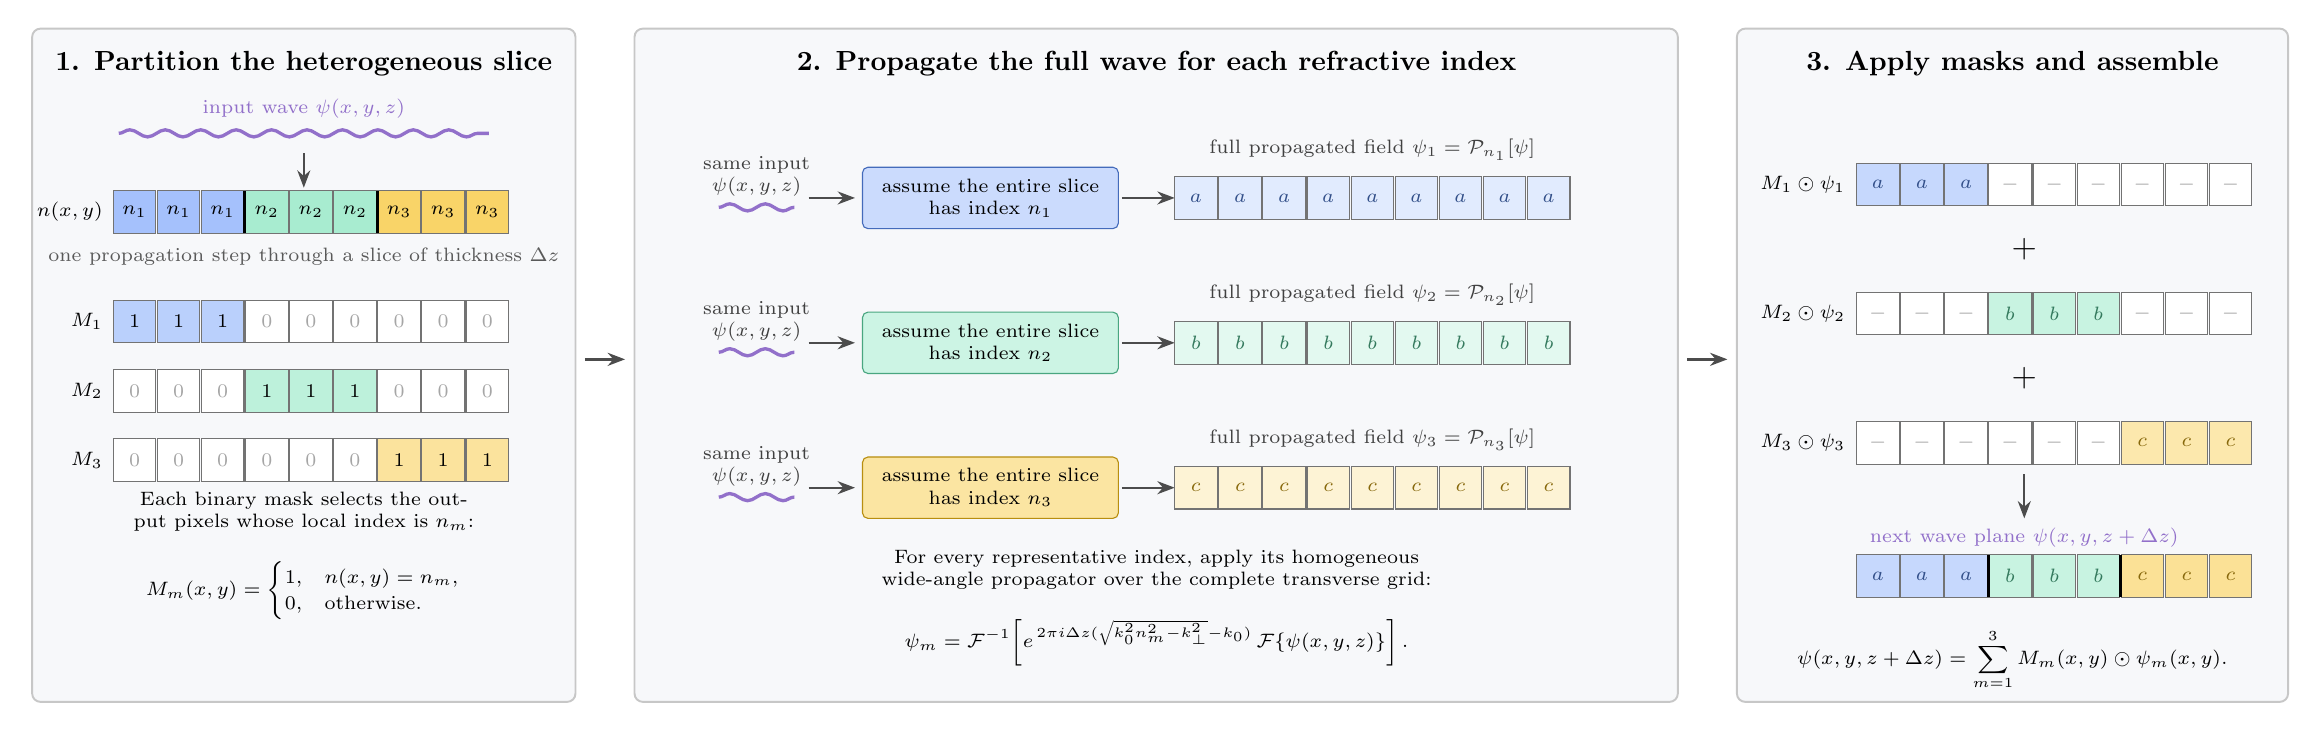
\begin{tikzpicture}[font=\sffamily]

    % Panel backgrounds.
    \begin{scope}[on background layer]
        \draw[panel] (-1.30,-0.35) rectangle (5.60,8.20);
        \draw[panel] (6.35,-0.35) rectangle (19.60,8.20);
        \draw[panel] (20.35,-0.35) rectangle (27.35,8.20);
    \end{scope}

    % -------------------------------------------------------------------------
    % 1. Build the masks from the local refractive-index map.
    % -------------------------------------------------------------------------
    \node[panel title] at (2.15,7.75) {1. Partition the heterogeneous slice};

    \node[font=\scriptsize, text=wavepurple] at (2.15,7.18)
        {input wave $\psi(x,y,z)$};
    \draw[wave] (-0.20,6.87) -- (4.50,6.87);
    \draw[flow] (2.15,6.62) -- (2.15,6.18);

    \node[anchor=east, font=\scriptsize] at (-0.28,5.87) {$n(x,y)$};
    \drawindexmap{0.00}{5.87}

    \node[font=\scriptsize, align=center, text=black!65] at (2.15,5.30)
        {one propagation step through a slice of thickness $\Delta z$};

    \node[anchor=east, font=\scriptsize] at (-0.28,4.48) {$M_1$};
    \drawmask{0.00}{4.48}{1}

    \node[anchor=east, font=\scriptsize] at (-0.28,3.60) {$M_2$};
    \drawmask{0.00}{3.60}{2}

    \node[anchor=east, font=\scriptsize] at (-0.28,2.72) {$M_3$};
    \drawmask{0.00}{2.72}{3}

    \node[align=center, font=\scriptsize, text width=5.7cm] at (2.15,1.50) {%
        Each binary mask selects the output pixels whose local index is $n_m$:
        \[
            M_m(x,y)=
            \begin{cases}
                1, & n(x,y)=n_m,\\
                0, & \text{otherwise.}
            \end{cases}
        \]
    };

    % -------------------------------------------------------------------------
    % 2. Propagate the complete input field once for each candidate index.
    % -------------------------------------------------------------------------
    \node[panel title] at (12.98,7.75)
        {2. Propagate the full wave for each refractive index};

    \node[branch label] at (7.90,6.32) {same input\\$\psi(x,y,z)$};
    \draw[wave] (7.42,5.93) -- (8.38,5.93);
    \draw[flow] (8.56,6.05) -- (9.15,6.05);
    \node[
        draw=indexone!75!black,
        fill=indexone!32,
        rounded corners=2pt,
        minimum width=3.25cm,
        minimum height=0.78cm,
        align=center,
        font=\scriptsize
    ] at (10.87,6.05) {assume the entire slice\\has index $n_1$};
    \draw[flow] (12.54,6.05) -- (13.21,6.05);
    \node[branch label] at (15.72,6.66) {full propagated field $\psi_1=\mathcal P_{n_1}[\psi]$};
    \drawfield{13.48}{6.05}{a}{indexone}

    \node[branch label] at (7.90,4.48) {same input\\$\psi(x,y,z)$};
    \draw[wave] (7.42,4.09) -- (8.38,4.09);
    \draw[flow] (8.56,4.21) -- (9.15,4.21);
    \node[
        draw=indextwo!75!black,
        fill=indextwo!32,
        rounded corners=2pt,
        minimum width=3.25cm,
        minimum height=0.78cm,
        align=center,
        font=\scriptsize
    ] at (10.87,4.21) {assume the entire slice\\has index $n_2$};
    \draw[flow] (12.54,4.21) -- (13.21,4.21);
    \node[branch label] at (15.72,4.82) {full propagated field $\psi_2=\mathcal P_{n_2}[\psi]$};
    \drawfield{13.48}{4.21}{b}{indextwo}

    \node[branch label] at (7.90,2.64) {same input\\$\psi(x,y,z)$};
    \draw[wave] (7.42,2.25) -- (8.38,2.25);
    \draw[flow] (8.56,2.37) -- (9.15,2.37);
    \node[
        draw=indexthree!75!black,
        fill=indexthree!40,
        rounded corners=2pt,
        minimum width=3.25cm,
        minimum height=0.78cm,
        align=center,
        font=\scriptsize
    ] at (10.87,2.37) {assume the entire slice\\has index $n_3$};
    \draw[flow] (12.54,2.37) -- (13.21,2.37);
    \node[branch label] at (15.72,2.98) {full propagated field $\psi_3=\mathcal P_{n_3}[\psi]$};
    \drawfield{13.48}{2.37}{c}{indexthree}

    \node[align=center, font=\scriptsize, text width=12.0cm] at (12.98,0.84) {%
        For every representative index, apply its homogeneous wide-angle
        propagator over the complete transverse grid:
        \[
            \psi_m =
            \mathcal F^{-1}\!\left[
                e^{\,2\pi i\Delta z(\sqrt{k_0^2 n_m^2-k_\perp^2}-k_0)}\,
                \mathcal F\{\psi(x,y,z)\}
            \right].
        \]
    };

    % -------------------------------------------------------------------------
    % 3. Select the locally appropriate output pixels and add them together.
    % -------------------------------------------------------------------------
    \node[panel title] at (23.85,7.75) {3. Apply masks and assemble};

    \node[anchor=east, font=\scriptsize] at (21.85,6.22) {$M_1\odot\psi_1$};
    \drawkept{22.14}{6.22}{1}{a}{indexone}

    \node[font=\large] at (24.00,5.40) {$+$};

    \node[anchor=east, font=\scriptsize] at (21.85,4.58) {$M_2\odot\psi_2$};
    \drawkept{22.14}{4.58}{2}{b}{indextwo}

    \node[font=\large] at (24.00,3.76) {$+$};

    \node[anchor=east, font=\scriptsize] at (21.85,2.94) {$M_3\odot\psi_3$};
    \drawkept{22.14}{2.94}{3}{c}{indexthree}

    \draw[flow] (24.00,2.54) -- (24.00,1.98);
    \node[font=\scriptsize, text=wavepurple] at (24.00,1.74)
        {next wave plane $\psi(x,y,z+\Delta z)$};
    \drawfinalfield{22.14}{1.25}

    \node[align=center, font=\scriptsize, text width=6.2cm] at (23.85,0.38) {%
        \[
            \psi(x,y,z+\Delta z)
            = \sum_{m=1}^{3} M_m(x,y)\odot\psi_m(x,y).
        \]
    };

    \draw[flow, line width=1.1pt] (5.72,4.00) -- (6.23,4.00);
    \draw[flow, line width=1.1pt] (19.72,4.00) -- (20.23,4.00);

\end{tikzpicture}
\end{document}
